\documentclass[10pt,twocolumn,letterpaper]{article}

\usepackage{cvpr}
\usepackage{times}
\usepackage{epsfig}
\usepackage{graphicx}
\usepackage{amsmath}
\usepackage{amssymb}

% Include other packages here, before hyperref.

% If you comment hyperref and then uncomment it, you should delete
% egpaper.aux before re-running latex.  (Or just hit 'q' on the first latex
% run, let it finish, and you should be clear).
\usepackage[breaklinks=true,bookmarks=false]{hyperref}

\cvprfinalcopy % *** Uncomment this line for the final submission

\def\cvprPaperID{****} % *** Enter the CVPR Paper ID here
\def\httilde{\mbox{\tt\raisebox{-.5ex}{\symbol{126}}}}

% Pages are numbered in submission mode, and unnumbered in camera-ready
%\ifcvprfinal\pagestyle{empty}\fi
\setcounter{page}{1}
\begin{document}

%%%%%%%%% TITLE
\title{Crowd Counting using fine tuning and density maps}

\author{Pierpaolo D'Odorico\\
{\tt\small pierpaolo.dodorico@studenti.unipd.it}
\and
Massimiliano Conte\\
{\tt\small massimiliano.conte@studenti.unipd.it}
}


\maketitle
%\thispagestyle{empty}
\begin{abstract}

This paper aims to investigate which is the best approach for crowd counting in a simple situation, among different computer vision tecniques. The counting is performed on images captured from a security camera placed in a shopping mall. In this simple but useful task the goal is to estimate the number of people that are present in the image. We can for example count the percentage of visitors who buyed from a specific shop or report to the mall staff that covid-19 social distancing laws are not respected. ttt

\end{abstract}

%%%%%%%%% BODY TEXT
\section{Introduction}

Crowd counting has been a challenge in recent years. The goal of this task is directly connected with crowd control and public safety. The affluence of people in different areas can be also useful for planning spaces and services. For example in our specific task we need to count people from seurity camera images in a mall, and this people counting can be useful for several business and safety applications. 
There were developed a lot of different tecniques for solving this computer vision task. Our idea is to compare two different tecniques and finding the best one for counting from single security camera images. The first approach is a convolutional neural network fine tuning on VGG16 network.  This very deep network was proposed by K. Simonyan and A. Zisserman from the University of Oxford and it was submitted to ImageNet challenge in 2014. The second approach deals with density maps. Those are useful in real life applications since the same number of people could have completely different crowd distributions. (as shown in Fig. 1). After implementing the two approaches on our problem we found that...


%------------------------------------------------------------------------
\section{Related work}

We based our project on informations contained in different papers about computer vision tasks and crowd counting. The first one is related to VGG16, the network we fine tuned for dealing with our people counting problem, and it is entitled “\textit{Very Deep Convolutional Networks for Large-Scale Image Recognition}” \cite{simonyan2014very}. In this paper the authors investigate the effect of the convolutional network depth on its accuracy in the
large-scale image recognition setting. In this convolutional neural networks they use very small (3x3) convolution filters, which shows that a significant improvement on the prior state of the art configurations. They also pushed the depth to 16-19 weight layers (Fig.\ref{fig:vgg16}). Those small convolutional filters can be useful in our application for finding people in images. Fine tuning the final layers and adding a regression one at the final part of the network, we hope that VGG16 model will achieve a good performance. 

\begin{figure}[h!]
  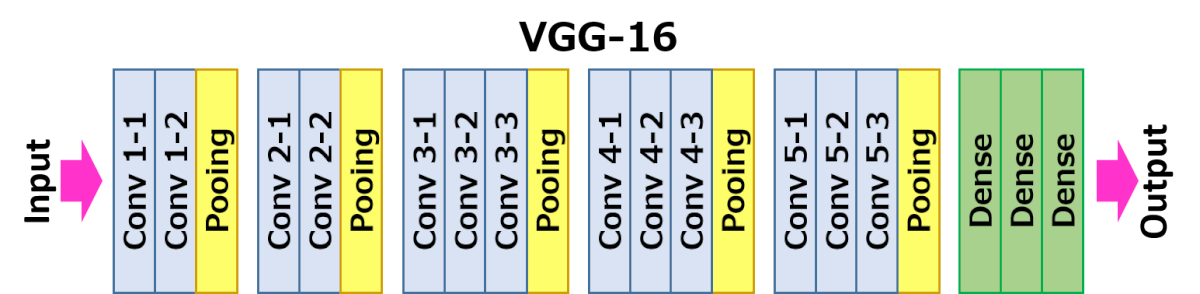
\includegraphics[width=\linewidth]{pics/vgg16.png}
  \caption{VGG16 deep CNN structure}
  \label{fig:vgg16}
\end{figure}

We relate also to two papers about density map crowd counting approach. The first one is entitled ”\textit{Single-Image Crowd Counting via Multi-Column Convolutional Neural Network}” \cite{zhang2016single}.

\begin{figure}[h!]
  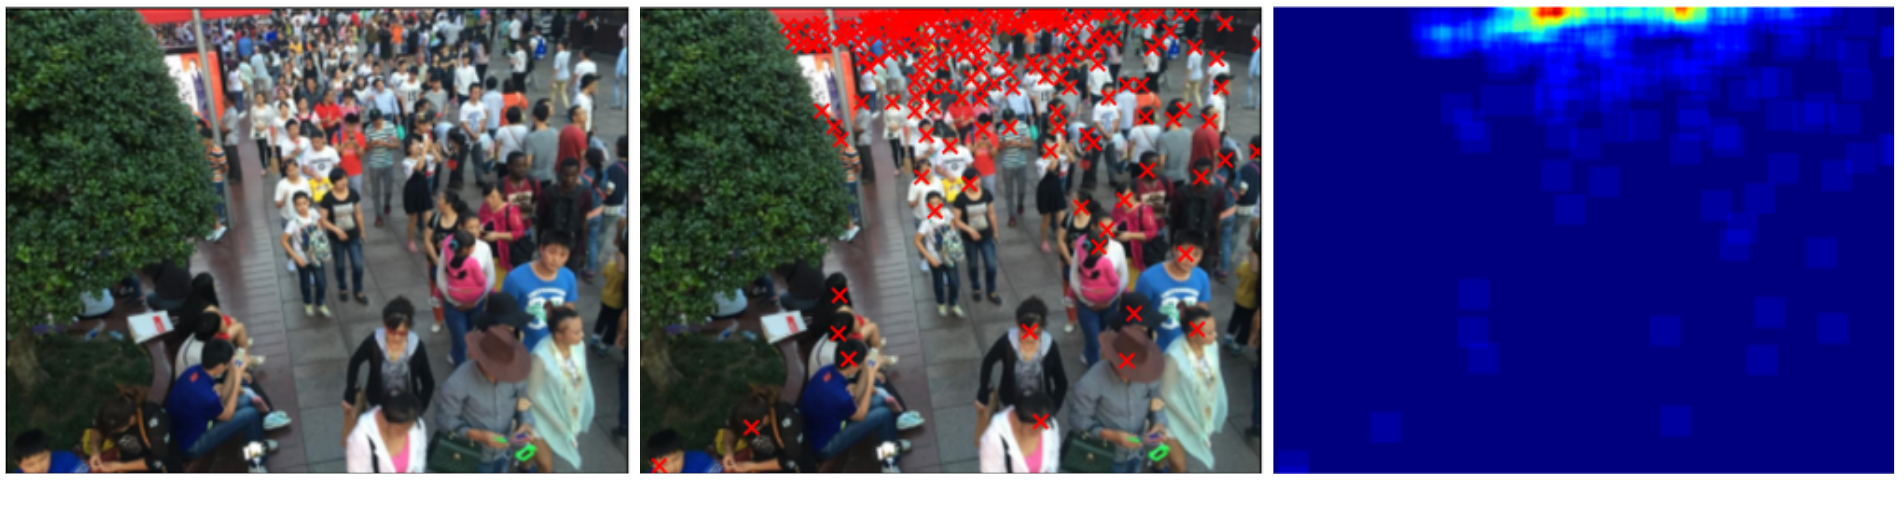
\includegraphics[width=\linewidth]{pics/densitymapapproach.png}
  \caption{Density map approach}
  \label{fig:densitymap}
\end{figure}
















%------------------------------------------------------------------------
\section{Formatting your paper}



%-------------------------------------------------------------------------
\subsection{Margins and page numbering}

All printed material, including text, illustrations, and charts, must be kept
within a print area 6-7/8 inches (17.5 cm) wide by 8-7/8 inches (22.54 cm)
high.
Page numbers should be in footer with page numbers, centered and .75
inches from the bottom of the page and make it start at the correct page
number rather than the 4321 in the example.  To do this fine the line (around
line 23)
\begin{verbatim}
%\ifcvprfinal\pagestyle{empty}\fi
\setcounter{page}{4321}
\end{verbatim}
where the number 4321 is your assigned starting page.

Make sure the first page is numbered by commenting out the first page being
empty on line 46
\begin{verbatim}
%\thispagestyle{empty}
\end{verbatim}


\subsection{References}

List and number all bibliographical references in 9-point Times,
single-spaced, at the end of your paper. When referenced in the text,
enclose the citation number in square brackets, for
example~\cite{Authors14}.  Where appropriate, include the name(s) of
editors of referenced books.

\begin{table}
\begin{center}
\begin{tabular}{|l|c|}
\hline
Method & Frobnability \\
\hline\hline
Theirs & Frumpy \\
Yours & Frobbly \\
Ours & Makes one's heart Frob\\
\hline
\end{tabular}
\end{center}
\caption{Results. Ours is better.}
\label{mytable}
\end{table}

%-------------------------------------------------------------------------
\subsection{Illustrations, graphs, and photographs}

All graphics should be centered.  Please ensure that any point you wish to make is resolvable in a printed copy of the paper.  Resize fonts in figures to match the font in the body text, and choose line widths which render effectively in print.  Many readers (and reviewers), even of an electronic copy, will choose to print your paper in order to read it.  You cannot
insist that they do otherwise, and therefore must not assume that they can
zoom in to see tiny details on a graphic.

When placing figures in \LaTeX, it's almost always best to use
\verb+\includegraphics+, and to specify the  figure width as a multiple of
the line width as in the example below
{\small\begin{verbatim}
   \usepackage[dvips]{graphicx} ...
   \includegraphics[width=0.8\linewidth]
                   {myfile.eps}
\end{verbatim}
}

{\small
\bibliographystyle{ieee_fullname}
\bibliography{egbib}
}

\end{document}
